\documentclass[12pt]{report}
\usepackage[utf8]{inputenc}
\usepackage[english, russian]{babel}
\usepackage{listings}
\usepackage{graphicx}
\usepackage{float}
\graphicspath{{imgs/}}
\usepackage{amsmath,amsfonts,amssymb,amsthm,mathtools} 
\usepackage{pgfplots}
\usepackage{filecontents}
\usepackage{indentfirst}
\usepackage{eucal}
\usepackage{enumitem}
\frenchspacing

\usepackage{indentfirst} % Красная строка

\usetikzlibrary{datavisualization}
\usetikzlibrary{datavisualization.formats.functions}

\usepackage{amsmath}
\usepackage{fixltx2e}
\usepackage{caption}


\definecolor{bluekeywords}{rgb}{0,0,1}
\definecolor{greencomments}{rgb}{0,0.5,0}
\definecolor{redstrings}{rgb}{0.64,0.08,0.08}
\definecolor{xmlcomments}{rgb}{0.5,0.5,0.5}
\definecolor{types}{rgb}{0.17,0.57,0.68}

\usepackage{listings}
\lstset{language=[Sharp]C,
	captionpos=t,
	numbers=left, %Nummerierung
	numberstyle=\small, % kleine Zeilennummern
	frame=single, % Oberhalb und unterhalb des Listings ist eine Linie
	stepnumber=1,                   
	numbersep=5pt,                
	showspaces=false,
	tabsize=2,
	showtabs=false,
	breaklines=true,
	showstringspaces=false,
	breakatwhitespace=true,
	escapeinside={(*@}{@*)},
	commentstyle=\color{greencomments},
	morekeywords={partial, var, value, get, set},
	keywordstyle=\color{bluekeywords},
	stringstyle=\color{redstrings},
	basicstyle=\ttfamily\small,
}

\usepackage[left=2cm,right=2cm, top=2cm,bottom=2cm,bindingoffset=0cm]{geometry}
% Для измененных титулов глав:
\usepackage{titlesec, blindtext, color} % подключаем нужные пакеты
\definecolor{gray75}{gray}{0.75} % определяем цвет
\newcommand{\hsp}{\hspace{20pt}} % длина линии в 20pt
% titleformat определяет стиль
\titleformat{\chapter}[hang]{\Huge\bfseries}{\thechapter\hsp\textcolor{gray75}{|}\hsp}{0pt}{\Huge\bfseries}


% plot
\usepackage{pgfplots}
\usepackage{filecontents}
\usetikzlibrary{datavisualization}
\usetikzlibrary{datavisualization.formats.functions}
 
\begin{document}
  %\def\chaptername{} % убирает "Глава"
\thispagestyle{empty}
\begin{titlepage}
	\noindent \begin{minipage}{0.15\textwidth}
	
\includegraphics[width=\linewidth]{b_logo}
	\end{minipage}
	\noindent\begin{minipage}{0.9\textwidth}\centering
		\textbf{Министерство науки и высшего образования Российской Федерации}\\
		\textbf{Федеральное государственное бюджетное образовательное учреждение высшего образования}\\
		\textbf{~~~«Московский государственный технический университет имени Н.Э.~Баумана}\\
		\textbf{(национальный исследовательский университет)»}\\
		\textbf{(МГТУ им. Н.Э.~Баумана)}
	\end{minipage}
	
	\noindent\rule{18cm}{3pt}
	\newline\newline
	\noindent ФАКУЛЬТЕТ $\underline{\text{«Информатика и системы управления»}}$ \newline\newline
	\noindent КАФЕДРА $\underline{\text{«Программное обеспечение ЭВМ и информационные технологии»}}$\newline\newline\newline\newline\newline\newline\newline\newline\newline\newline\newline
	
	
	\begin{center}
		\noindent\begin{minipage}{1.3\textwidth}\centering
			\Large\textbf{  Отчет по лабораторной работе №2}\newline
			\textbf{по дисциплине "Анализ алгоритмов"}\newline\newline
		\end{minipage}
	\end{center}
	
	\noindent\textbf{Тема} $\underline{\text{Анализ алгоритмов умножения матриц}}$\newline\newline
	\noindent\textbf{Студент} $\underline{\text{Малышев И. А.}}$\newline\newline
	\noindent\textbf{Группа} $\underline{\text{ИУ7-51Б}}$\newline\newline
	\noindent\textbf{Оценка (баллы)} $\underline{\text{~~~~~~~~~~~~~~~~~~~~~~~~~~~}}$\newline\newline
	\noindent\textbf{Преподаватель: } $\underline{\text{Волкова Л. Л.}}$\newline\newline\newline
	
	\begin{center}
		\vfill
		Москва~---~\the\year
		~г.
	\end{center}
\end{titlepage}


\renewcommand{\contentsname}{Содержание}
\tableofcontents
  
\newpage
\chapter*{Введение}
\addcontentsline{toc}{chapter}{Введение}

Матрица -- математический объект, эквивалентный двумерному массиву. Числа располагаются в матрице по строкам и столбцам. Две матрицы одинакового размера можно поэлементно сложить или вычесть друг из друга. Если число столбцов в первой матрице совпадает с числом строк во второй, то эти две матрицы можно перемножить[1].

Умножение матриц -- это один из базовых алгоритмов, который широко применяется в численных методах, в частности, в машинном обучении, в компьютерной графике для реализации афинных преобразований. Именно поэтому важно, чтобы алгоритм был максимально эффективен по затрачиваемым ресурсам. 

Именно поэтому \textbf{целью} данной работы является изучение алгоритмов умножения матриц, в частности: обычный алгоритм, алгоритм Винограда и оптимизированный алгоритм Винограда. 

Для достижения поставленной цели необходимо решить следующие задачи.
\begin{enumerate}
	\item Изучить три существующих алгоритма умножения матриц: обычный, Винограда, оптимизированный Винограда.
	\item Разработать и привести схемы алгоритмов.
	\item Оценить трудоёмкость алгоритмов на основе расчетов в выбранной модели вычислений.
	\item Определить средства для реализации алгоритмов и реализовать их.
	\item Оценить трудоёмкость алгоритмов на основе экспериментальных данных.
\end{enumerate}


\chapter{Аналитическая часть}

В этом разделе приведён обзор и анализ алгоритмов умножения матриц.

\section{Стандартный алгоритм}

Пусть даны две прямоугольные матрицы:
\begin{equation}
	A_{lm} = \begin{pmatrix}
		a_{11} & a_{12} & \ldots & a_{1m}\\
		a_{21} & a_{22} & \ldots & a_{2m}\\
		\vdots & \vdots & \ddots & \vdots\\
		a_{l1} & a_{l2} & \ldots & a_{lm}
	\end{pmatrix},
	\quad
	B_{mn} = \begin{pmatrix}
		b_{11} & b_{12} & \ldots & b_{1n}\\
		b_{21} & b_{22} & \ldots & b_{2n}\\
		\vdots & \vdots & \ddots & \vdots\\
		b_{m1} & b_{m2} & \ldots & b_{mn}
	\end{pmatrix},
\end{equation}

Тогда матрица $C$
\begin{equation}
	C_{ln} = \begin{pmatrix}
		c_{11} & c_{12} & \ldots & c_{1n}\\
		c_{21} & c_{22} & \ldots & c_{2n}\\
		\vdots & \vdots & \ddots & \vdots\\
		c_{l1} & c_{l2} & \ldots & c_{ln}
	\end{pmatrix},
\end{equation}

, где
\begin{equation}
	\label{eq:M}
	c_{ij} =
	\sum_{r=1}^{m} a_{ir}b_{rj} \quad (i=\overline{1,l}; j=\overline{1,n})
\end{equation}

будет называться произведением матриц $A$ и $B$.
Стандартный алгоритм реализует данную формулу.

\section{Алгоритм Винограда}

Если посмотреть на результат умножения двух матриц, то видно, что каждый элемент в нем представляет собой скалярное произведение соответствующих строки и столбца исходных матриц.
Можно заметить также, что такое умножение допускает предварительную обработку, позволяющую часть работы выполнить заранее [1].

Рассмотрим два вектора $V = (v_1, v_2, v_3, v_4)$ и $W = (w_1, w_2, w_3, w_4)$.
Их скалярное произведение равно: $V \cdot W = v_1w_1 + v_2w_2 + v_3w_3 + v_4w_4$, что эквивалентно (\ref{for:new}):
\begin{equation}
	\label{for:new}
	V \cdot W = (v_1 + w_2)(v_2 + w_1) + (v_3 + w_4)(v_4 + w_3) - v_1v_2 - v_3v_4 - w_1w_2 - w_3w_4.
\end{equation}

Несмотря на то, что второе выражение требует вычисления большего количества операций, чем стандартный алгоритм: вместо четырёх умножений - шесть, а вместо трёх сложений - десять, выражение в правой части последнего равенства допускает предварительную обработку: его части можно вычислить заранее и запомнить для каждой строки первой матрицы и для каждого столбца второй, что позволит для каждого элемента выполнять лишь два умножения и пять сложений, складывая затем только лишь с 2 предварительно посчитанными суммами соседних элементов текущих строк и столбцов.
Из-за того, что операция сложения быстрее операции умножения в ЭВМ, на практике алгоритм должен работать быстрее стандартного.

\section{Оптимизированный алгоритм Винограда}

Оптимизация алгоритма заключается в следующем:
\begin{itemize}
	\item в начале происходят предвычисления с помощью двух циклов, которые можно поместить в один, что уменьшит вклад циклов в трудоёмкость;
	\item в каждом из циклов приходится производить умножение на 2 при индексации, чтобы это исправить можно увеличить шаг с единицы на двойку и границу цикла вдвое.
\end{itemize}

\section{Вывод}

В данном разделе были рассмотрены алгоритмы классического умножения матриц и алгоритм Винограда. Было выявлено, что алгоритм Винограда отличается от стандартного наличием предварительной обработки строк и столбцов, что позволяет сократить количество умножений, а значит ускорить алгоритм.
	
\newpage

\chapter{Конструкторская часть}

В этом разделе приводятся схемы алгоритмов умножения матриц, приведённых в аналитической части, и расчёты их трудоёмкости. 

\section{Схемы алгоритмов}

На рисунках \ref{std}, \ref{vin} и \ref{optvin} показаны схемы алгоритмов сортировки пузырьком, выбором и быстрой сортировки соответственно.

\begin{figure}[H]
	\centering
	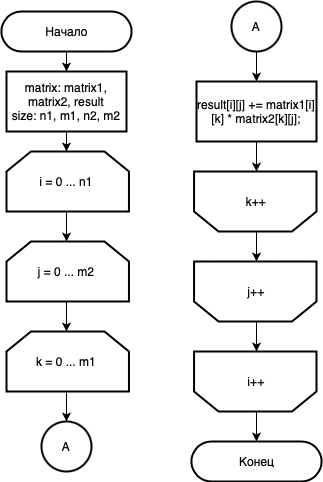
\includegraphics[scale = 0.75]{base.drawio.png}
	\caption{Схема стандартного алгоритма}
	\label{std}
\end{figure}

\begin{figure}[H]
	\centering
	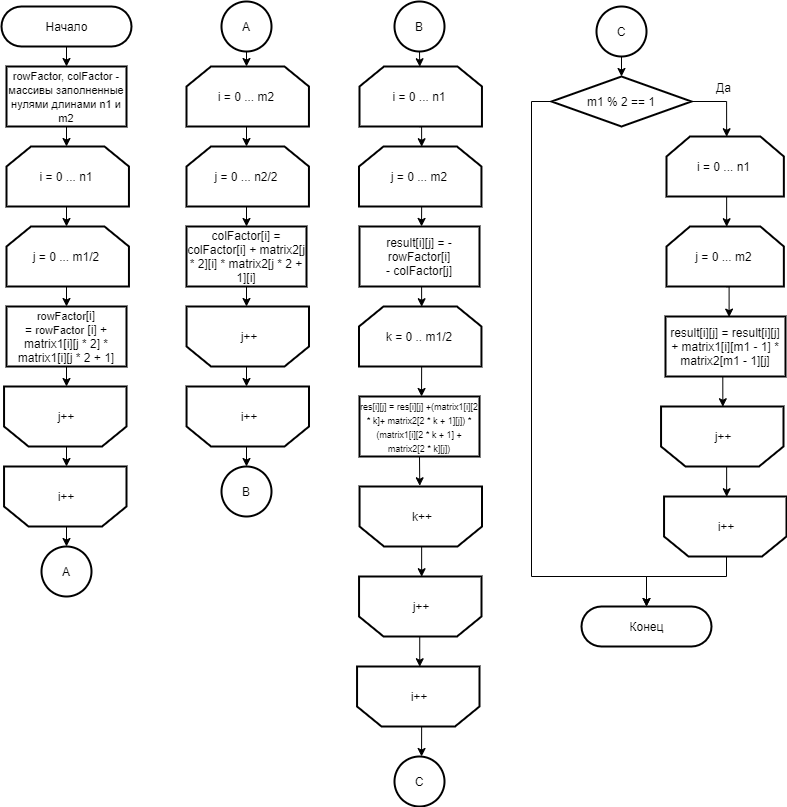
\includegraphics[scale = 0.65]{vin.drawio.png}
	\caption{Схема алгоритма Винограда}
	\label{vin}
\end{figure}

\begin{figure}[H]
	\centering
	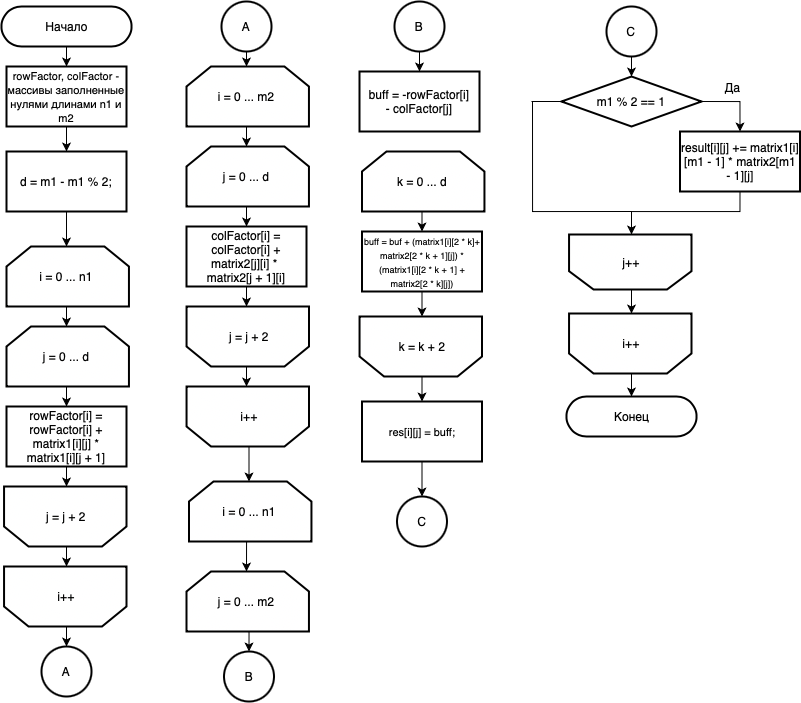
\includegraphics[scale=0.65]{vinOpt.drawio.png}
	\caption{Схема оптимизированного алгоритма Винограда}
	\label{optvin}
\end{figure}


\section{Модель вычислений}

Для последующего вычисления трудоемкости введём модель вычислений [2]:

\begin{enumerate}
	\item Операции из списка (\ref{for:opers}) имеют трудоемкость 1.
	\begin{equation}
		\label{for:opers}
		+, -, /, \%, ==, !=, <, >, <=, >=, [], ++, {-}-
	\end{equation}
	\item Трудоемкость оператора выбора if условие then A else B рассчитывается, как (\ref{for:if}).
	\begin{equation}
		\label{for:if}
		f_{if} = f_{\text{условия}} +
		\begin{cases}
			f_A, & \text{если условие выполняется,}\\
			f_B, & \text{иначе.}
		\end{cases}
	\end{equation}
	\item Трудоемкость цикла рассчитывается, как (\ref{for:for}).
	\begin{equation}
		\label{for:for}
		f_{for} = f_{\text{инициализации}} + f_{\text{сравнения}} + N(f_{\text{тела}} + f_{\text{инкремента}} + f_{\text{сравнения}})
	\end{equation}
	\item Трудоемкость вызова функции равна 0.
\end{enumerate}

\section{Трудоёмкость алгоритмов}
Примем, что размеры первой матрицы (r, s), а второй - (s, c).
\subsection{Стандартный алгоритм умножения матриц}

Трудоёмкость стандартного алгоритма в выбранной модели вычислений в худшем и лучшем случаях рассчитывается следующим образом:
\begin{equation}
	f_{base} = 2 + r(2 + 2 + c(2 + 2 + s(2 + 11))) = 13scr + 4cr + 4r + 2
\end{equation}

\subsection{Алгоритм Винограда}
Для алгоритма Винограда худшим случаем являются матрицы с нечётным общим размером, а лучшим - с чётным, из-за того что отпадает необходимость в последнем цикле.

Трудоёмкость алгоритма Винограда является суммой трудоёмкостей следующих последовательно выполненных действий:
\begin{enumerate}
	
	\item Заполнения вектора rowFactor:
	\begin{equation}
		f_{rowFactor} = 3 + r(2 + 2 + \frac{s}{2}(2 + 11)) = 6.5sr + 4r + 3;
	\end{equation}
	
	\item Заполнения вектора colFactor:
	\begin{equation}
		f_{colFactor} = 2 + c(2 + 2 + \frac{s}{2}(2 + 11)) = 6.5sc + 4r + 2;
	\end{equation}
	
	\item Основного цикла заполнения матрицы:
	\begin{equation}
		f_{cycle} = 2 + r(2 + 2 + c(2 + 2 + 7 + \frac{s}{2}(2 + 23))) = 12.5scr + 11cr + 4r + 2;
	\end{equation}
	
	\item Цикла для дополнения умножения, если общий размер нечётный:
	\begin{equation}
		f_{last} = \begin{cases}
			2, & \text{чётная,}\\
			2 + 2 + r(2 + 2 + c(2 + 13)) = 15cr + 4r + 4, & \text{иначе.}
		\end{cases}
	\end{equation}
\end{enumerate}
Итак, для лучшего случая (чётный размер матриц): 
\begin{equation}
	f_{vin\_b} = 6.5sr + 4r + 3 + 6.5sc + 4r + 2 + 12.5scr + 11cr + 4r + 2 + 2 = 12.5scr + 6.5sr + 6.5sc + 11cr + 12r + 9;
\end{equation}

Для худшего случая (нечётный общий размер матриц): 
\begin{eqnarray}
	f_{vin\_w} = 6.5sr + 4r + 3 + 6.5sc + 4r + 2 + 12.5scr + 11cr + 4r + 2 + 15cr + 4r + 4 =\\ = 12.5scr + 6.5sr + 6.5sc + 26cr + 16r + 11;
\end{eqnarray}

\subsection{Оптимизированный алгоритм Винограда}

Трудоёмкость оптимизированного алгоритма Винограда является суммой трудоёмкостей следующих последовательно выполненных действий:
\begin{enumerate}
	\item Заполнения вектора rowFactor:
	\begin{equation}
		f_{rowFactor} = 5 + r(3 + 2 + \frac{s}{2}(3 + 10)) = 6.5sr + 5r + 5;
	\end{equation}
	
	\item Заполнения вектора colFactor:
	\begin{equation}
		f_{colFactor} = 2 + c(2 + 2 + \frac{s}{2}(2 + 11)) = 6.5sс + 5r + 2;
	\end{equation}
	
	\item Основного цикла заполнения матрицы:
	\begin{equation}
		f_{cycle} = 3 + 2 + r(2 + 2 + c(2 + 2 + 5 + \frac{s}{2}(3 + 15) + f_{last} + 3)) = 9scr + 12cr + f_{last}cr + 4r + 5
	\end{equation}
	\begin{equation}
		f_{last} = \begin{cases}
			0, & \text{чётная,}\\
			9, & \text{иначе.}
		\end{cases}
	\end{equation}
\end{enumerate}

Итак, для лучшего случая (чётный размер матриц): 
\begin{equation}
	f_{vinOpt\_b} = 6.5sr + 5r + 5 + 6.5sс + 5r + 2 + 9scr + 12cr + 4r + 5 = 9scr + 6.5sr + 6.5sc + 12cr + 14r + 12;
\end{equation}

Для худшего случая (нечётный общий размер матриц): 
\begin{equation}
	f_{vinOpt\_w} = 6.5sr + 5r + 5 + 6.5sс + 5r + 2 + 9scr + 12cr + 9cr + 4r + 5 = 9scr + 6.5sr + 6.5sc + 21cr + 14r + 12;
\end{equation}

\section{Вывод}
На основе теоретических данных, полученных из аналитического раздела, были построены схемы алгоритмов умножения матриц, оценены их трудоёмкости в лучшем и худшем случаях.

\newpage

\chapter{Технологическая часть}
В данном разделе приводится реализация алгоритмов, схемы которых были разработаны в конструкторской части. Кроме того, обосновывается выбор технологического стека и проводится тестирование реализованных алгоритмов.

\section{Средства реализации}

В качестве языка программирования был выбран C\#, а среду разработки -- Visual Studio, т. к. я знаком с данным языком и имею представление о тестировании программ в данном языке. Время работы алгоритмов было замерено с помощью библиотеки System.Diagnostics, класса Stopwatch, который имеет методы для расчёта процессорного времени [3].


\section{Реализация алгоритмов}

В листингах 3.1 - 3.3 приведена реализация трёх алгоритмов умножения матриц.

\captionsetup{singlelinecheck = false, justification=raggedright}
\begin{lstlisting}[label=base_code,caption=Функция обычного алгоритма умножения матриц]
public Matrix MultiplyStandart(Matrix a)
{
	Matrix result = new Matrix(n, a.M);
	
	for (int i = 0; i < n; i++)
	{
		for (int k = 0; k < a.M; k++)
		{
			result[i, k] = 0;
			for (int j = 0; j < m; j++)
			result[i, k] += this[i, j] * a[j, k];
		}
	}
	
	return result;
}
\end{lstlisting}
\newpage
\begin{lstlisting}[label=vin_code,caption=Функция алгоритма умножения матриц Винограда]
public Matrix MultiplyVinograd(Matrix matr)
{
	Matrix result = new Matrix(n, matr.M);
	double[] rowFactor = new double[n];
	double[] colFactor = new double[matr.M];
	
	int d = m / 2;
	for (int i = 0; i < n; i++)
	{
		rowFactor[i] = this[i, 0] * this[i, 1];
		for (int j = 1; j < d; j++)
			rowFactor[i] = rowFactor[i] + this[i, 2 * j] * this[i, 2 * j + 1];
	}
	
	for (int i = 0; i < matr.M; i++)
	{
		colFactor[i] = matr[0, i] * matr[1, i];
		for (int j = 1; j < d; j++)
			colFactor[i] = colFactor[i] + matr[2 * j, i] * matr[2 * j + 1, i];
	}
	
	for (int i = 0; i < n; i++)
	{
		for (int j = 0; j < matr.M; j++)
		{
			result[i, j] = -rowFactor[i] - colFactor[j];
			for (int k = 0; k < d; k++)
				result[i, j] = result[i, j] + (this[i, 2 * k] + matr[2 * k + 1, j]) * (this[i, 2 * k + 1] + matr[2 * k, j]);
		}
	}
	
	if (m % 2 == 1)
	{
		for (int i = 0; i < n; i++)
			for (int j = 0; j < matr.M; j++)
				result[i, j] = result[i, j] + this[i, n - 1] * matr[n - 1, j];
	}
	
	return result;
}
\end{lstlisting}
\newpage
\begin{lstlisting}[label=vin_opt_code,caption=Функция оптимизированного алгоритма умножения матриц Винограда]
public Matrix MultiplyVinogradOptimised(Matrix matr)
{
	Matrix result = new Matrix(n, matr.M);
	double[] rowFactor = new double[n];
	double[] colFactor = new double[matr.M];
	
	for (int i = 0; i < n; i++)
	{
		rowFactor[i] = colFactor[i] = 0;
		for (int j = 0; j < m - 1; j += 2)
		{
			rowFactor[i] += this[i, j] * this[i, j + 1];
			colFactor[i] += matr[j, i] * matr[j + 1, i];
		}
	}
	
	for (int i = 0; i < n; i++)
	for (int j = 0; j < matr.M; j++)
	{
		double res = -rowFactor[i] - colFactor[j];
		for (int k = 0; k < m - 1; k += 2)
			res += (this[i, k] + matr[k + 1, j]) * (this[i, k + 1] + matr[k, j]);
		
		result[i, j] = res;
	}
	
	if (m % 2 != 0)
	for (int i = 0; i < n; i++)
	for (int j = 0; j < matr.M; j++)
		result[i, j] += this[i, m - 1] * matr[matr.N - 1, j];
	
	return result;
}
\end{lstlisting}
\captionsetup{singlelinecheck = false, justification=centering}
\newpage
\section{Тестирование}

В таблице~\ref{tabular:test_rec} приведены тесты для функций, реализующих стандартный алгоритм умножения матриц, алгоритм Винограда и оптимизированный алгоритм Винограда.

\begin{table}[H]
	\begin{center}
		\begin{tabular}{c@{\hspace{7mm}}c@{\hspace{7mm}}c@{\hspace{7mm}}c@{\hspace{7mm}}}
			\hline
			Первая матрица & Вторая матрица & Ожидаемый результат & Фактический результат \\
			\hline
			\vspace{4mm}
			$\begin{pmatrix}
				1 & 2 & 3\\
				3 & 4 & 5
			\end{pmatrix}$ &
			$\begin{pmatrix}
				2 & 3 & 7\\
				5 & 1 & 10\\
				6 & -1 & 4
			\end{pmatrix}$ &
			$\begin{pmatrix}
				30 & 2 & 39 \\
				56 & 8 & 81 
			\end{pmatrix}$ &
			$\begin{pmatrix}
				30 & 2 & 39 \\
				56 & 8 & 81 
			\end{pmatrix}$ \\
			\vspace{2mm}
			\vspace{2mm}
			$\begin{pmatrix}
				1 & 2\\
				3 & 4
			\end{pmatrix}$ &
			$\begin{pmatrix}
				2 & 3 & 7\\
				5 & 1 & 10
			\end{pmatrix}$ &
			$\begin{pmatrix}
				12 & 5 & 27 \\
				26 & 13 & 61 
			\end{pmatrix}$ &
			$\begin{pmatrix}
				12 & 5 & 27 \\
				26 & 13 & 61 
			\end{pmatrix}$ \\
			\vspace{2mm}
			\vspace{2mm}
			$\begin{pmatrix}
				2
			\end{pmatrix}$ &
			$\begin{pmatrix}
				2
			\end{pmatrix}$ &
			$\begin{pmatrix}
				4
			\end{pmatrix}$ &
			$\begin{pmatrix}
				4
			\end{pmatrix}$ \\
			\vspace{2mm}
			\vspace{2mm}
			$\begin{pmatrix}
				1 & -2 & 3\\
				1 & 2 & 3\\
				1 & 2 & 3
			\end{pmatrix}$ &
			$\begin{pmatrix}
				-1 & 2 & 3\\
				1 & 2 & 3\\
				1 & 2 & 3
			\end{pmatrix}$ &
			$\begin{pmatrix}
				0 & 4 & 6\\
				4 & 12 & 18\\
				4 & 12 & 18
			\end{pmatrix}$ &
		$\begin{pmatrix}
			0 & 4 & 6\\
			4 & 12 & 18\\
			4 & 12 & 18
		\end{pmatrix}$ \\
		\end{tabular}
	\end{center}
	\caption{\label{tabular:test_rec} Тестирование функций}
\end{table}
Все тесты пройдены успешно.
\section{Вывод}

В данном разделе были реализованы алгоритмы умножения матриц: обычный алгоритм, алгоритм Винограда и оптимизированный алгоритм Винограда. Кроме того, реализации были успешно протестированы.

\newpage

\chapter{Исследовательская часть}

В данном разделе проводится сравненительный анализ реализованных алгоритмов по процессорному времени.

\section{Технические характеристики}

Ниже приведены технические характеристики устройства, на котором было проведено тестирование ПО:

\begin{itemize}
	\item Операционная система: Windows 10 Home 64-bit [4];
	\item Оперативная память: 16 GB;
	\item Процессор: 4.0 GHz 4‑ядерный процессор Intel Core i7-4790K [5].

\end{itemize}

\section{Время выполнения реализаций алгоритмов}

Для сравнительного анализа времени выполнения реализаций алгоритмов был проведен эксперимент. Для замеров были сформированы следующие пары квадратных матриц:
\begin{itemize}
	\item порядок матриц чётный и варьируется в пределах от 100 до 1100 с шагом 100;
	\item порядок матриц нечётный и варьируется в пределах от 1001 до 2101 с шагом 100.
\end{itemize}

В таблицах \ref{timeEven} и \ref{timeOdd} представлены результаты замеров. Время измерялось 10 раз для каждой пары матриц, после усреднялось. 

\begin{table} [H]
	\label{timeEven}
	\caption{Таблица времени выполнения (в секундах) алгоритмов при чётных размерах}
	\begin{center}
		\begin{tabular}{|c c c c|} 
			\hline
			Размер матрицы & Стандартный & Виноград & Оптимизированный \\  
			\hline
			100 & 0.024 & 0.014 & 0.009 \\
			\hline
			200 & 0.17 & 0.106 & 0.075 \\
			\hline
			300 & 0.527 & 0.386 & 0.29 \\
			\hline
			400 & 1.476 & 0.961 & 0.642 \\
			\hline
			500 & 3.162 & 2.055 & 1.296 \\
			\hline
			600 & 5.463 & 4.036 & 2.314 \\
			\hline
			700 & 9.451 & 6.788 & 4.836 \\
			\hline
			800 & 14.027 & 9.366 & 5.86 \\
			\hline
			900 & 18.884 & 14.12 & 11.594 \\
			\hline
			1000 & 26.829 & 18.049 & 13.348 \\
			\hline
		\end{tabular}
	\end{center}
\end{table}

\begin{figure}[H]
	\centering
	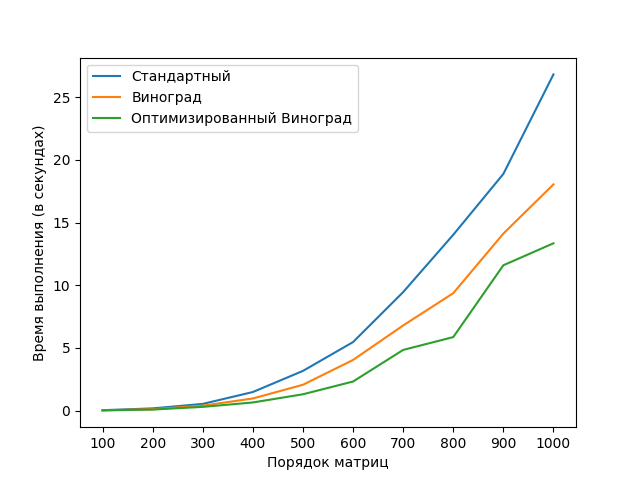
\includegraphics[scale=0.8]{even.png}
	\caption{Зависимость времени умножения квадратных матриц чётного порядка от величины порядка}
	\label{evenGraph}
\end{figure}

\begin{table} [H]
	\label{timeOdd}
	\caption{Таблица времени выполнения (в секундах) алгоритмов при нечётных размерах}
	\begin{center}
		\begin{tabular}{|c c c c|} 
			\hline
			Размер матрицы & Стандартный & Виноград & Оптимизированный \\  
			\hline
			101 & 0.020 & 0.013 & 0.009 \\
			\hline
			201 & 0.158 & 0.108 & 0.072 \\
			\hline
			301 & 0.536 & 0.393 & 0.246 \\
			\hline
			401 & 1.337 & 0.954 & 0.604 \\
			\hline
			501 & 2.807 & 1.835 & 1.253 \\
			\hline
			601 & 4.945 & 3.405 & 2.124 \\
			\hline
			701 & 8.353 & 5.441 & 3.573 \\
			\hline
			801 & 13.452 & 9.147 & 5.968 \\
			\hline
			901 & 18.569 & 14.258 & 9.55 \\
			\hline
			1001 & 26.865 & 21.295 & 16.106 \\
			\hline
		\end{tabular}
	\end{center}
\end{table}

\begin{figure}[H]
	\centering
	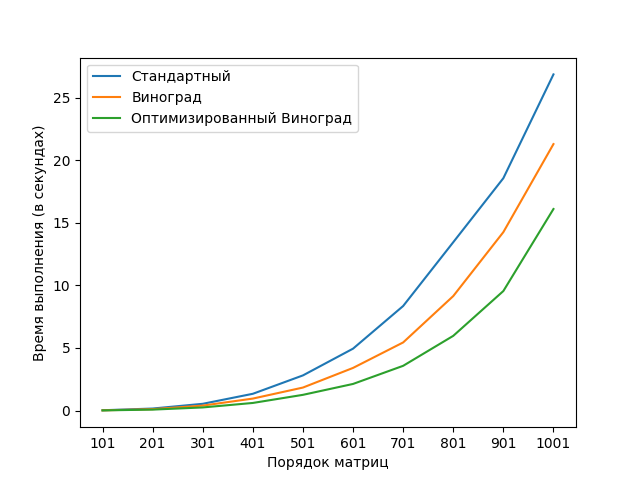
\includegraphics[scale=0.8]{odd.png}
	\caption{Зависимость времени умножения квадратных матриц нечётного порядка от величины порядка}
	\label{oddGraph}
\end{figure}

\section{Вывод}

На основе замеров процессорного времени было получено, что алгоритм Винограда в среднем в 1.4-1.7 раз быстрее, чем обычный алгоритм умножения матриц и немного хуже оптимизированного.

Также выявлено, что матрицы нечётного порядка перемножаются немного медленее, т. к. время тратится ещё и на обработку последнего столбца.


\chapter*{Заключение}
\addcontentsline{toc}{chapter}{Заключение}

В рамках данной лабораторной работы:

\begin{itemize}
	\item были изучены и реализованы 3 алгоритма умножения матриц: обычный, Винограда, оптимизированный Винограда;
	\item был произведён анализ трудоёмкости алгоритмов на основе теоретических расчётов и выбранной модели вычислений;
	\item был сделан сравнительный анализ алгоритмов на основе экспериментальных данных.
\end{itemize}

На основании анализа трудоёмкости алгоритмов в выбранной модели вычислений было показано, что улучшенный алгоритм Винограда имеет меньшую сложность, нежели простой алгоритм умножения матриц. На основании замеров времени исполнения алгоритмов, был сделан вывод о том, что алгоритм Винограда в среднем в 1.4-1.7 раз быстрее, чем обычный алгоритм умножения матриц и немного хуже оптимизированного. При этом матрицы нечётного порядка перемножаются немного медленее, чем чётного. 

Поставленная цель была достигнута.

\chapter*{Список литературы}
\addcontentsline{toc}{chapter}{Список литературы}
\begin{enumerate}
	\item Дж. Макконнелл. Основы современных алгоритмов. 2-е дополненное издание, Москва: Техносфера, 2004. - 368с. ISBN 5-94836-005-9

	\item Абрамов С. А. Лекции о сложности алгоритмов. - М., МЦНМО, 2020. - Изд. 3-е, испр. и доп. - 256 с. - ISBN: 978-5-443-91464-0
	\item Свойство Process.UserProcessorTime [Электронный ресурс]. Режим доступа: https://docs.microsoft.com/ru-ru/dotnet/api/system.diagnostics.stopwatch?view=net-5.0. Дата обращения: 02.10.2021
	\item Windows 10 [Электронный ресурс]. Режим доступа: https://www.microsoft.com/ru-ru/windows/get-windows-10. Дата обращения: 02.10.2021
	\item Процессор Intel Core I7-4790K [Электронный ресурс]. Режим доступа: https://ark.intel.com/content/www/ru/ru/ark/products/80807/intel-core-i7-4790k-processor-8m-cache-up-to-4-40-ghz.html. Дата обращения: 02.10.2021
\end{enumerate}


\end{document}